\documentclass[12pt, a4paper]{article}
% --- Packages ---
\usepackage[utf8]{inputenc}
\usepackage[T1]{fontenc}
\usepackage{geometry}
\geometry{top=2.5cm, bottom=2.5cm, left=2.5cm, right=2.5cm}
\usepackage{amsmath, amssymb, amsthm}
\usepackage{graphicx}
\usepackage{enumitem}
\usepackage{xcolor}
\usepackage{tikz}
\usetikzlibrary{shapes, arrows, positioning, calc, trees, backgrounds}
\usepackage[most]{tcolorbox}
\usepackage{hyperref}
\usepackage{float}
\usepackage{fancyhdr}

% --- Colors ---
\definecolor{deepblue}{RGB}{0, 51, 102}
\definecolor{lightgray}{RGB}{240, 240, 240}
\definecolor{accentcolor}{RGB}{204, 0, 0}

% --- Custom Environments ---
\newtcolorbox[auto counter]{problem}[2][]{%
    colback=white,
    colframe=deepblue,
    coltitle=white,
    fonttitle=\bfseries\large,
    title=Problem \thetcbcounter: #2,
    sharp corners,
    boxrule=0.8mm,
    #1
}

\newtcolorbox{solution}{%
    colback=lightgray!30,
    colframe=accentcolor!80,
    coltitle=white,
    fonttitle=\bfseries,
    title=Step-by-Step Solution,
    sharp corners=south,
    boxrule=0.5mm,
    breakable
}

\newtcolorbox{concept}[1][]{%
    colback=yellow!10,
    colframe=orange!80!black,
    title=Key Concept,
    fonttitle=\bfseries,
    #1
}

% --- Header/Footer ---
\pagestyle{fancy}
\fancyhf{}
\lhead{\textbf{Deep Reinforcement Learning}}
\rhead{Advanced Practice Guide}
\cfoot{\thepage}

% --- TikZ Styles ---
\tikzset{
    state/.style={circle, draw, minimum size=1cm, fill=blue!10, thick},
    action/.style={circle, draw, minimum size=0.5cm, fill=red!10, thick},
    netnode/.style={circle, draw, minimum size=0.8cm, fill=green!10},
    arrow/.style={->, >=stealth, thick},
    box/.style={rectangle, draw, minimum width=2cm, minimum height=1cm, fill=white, thick}
}

% --- Title Info ---
\title{\textbf{Deep Reinforcement Learning Scenario-Based Practice Guide}\\
\large 10 distinct and numerical types problems}
\author{Comprehensive Exam Preparation}
\date{\today}

\begin{document}

\maketitle

\section*{Introduction}
This practice guide contains 10 distinct, advanced numerical problems covering the full spectrum of Deep Reinforcement Learning. Unlike standard textbook examples, these problems are framed as real-world scenarios (e.g., ad optimization, autonomous driving, server load balancing) requiring careful formulation and multi-step calculations. The difficulty is aligned with comprehensive exams, emphasizing Deep RL concepts (DQN, Policy Gradients, PPO, AlphaZero) while ensuring a solid foundation in classic MDPs and Bandits.

\tableofcontents
\newpage

% --- Problem 1: Bandits (UCB) ---
\begin{problem}{Ad Campaign Optimization (Non-Stationary UCB)}
\textbf{Scenario:}
An online advertising platform uses a Multi-Armed Bandit algorithm to select which ad creative (banner) to display to users. There are 3 available creatives: $\{A, B, C\}$. The platform uses the Upper Confidence Bound (UCB) algorithm to balance exploration and exploitation. However, user preferences are non-stationary (they change over time).

Let $Q_t(a)$ be the estimated click-through rate (CTR) for ad $a$ at time $t$, and $N_t(a)$ be the number of times ad $a$ has been shown up to time $t$. The UCB score is calculated as:
\[ UCB_t(a) = Q_t(a) + c \sqrt{\frac{\ln t}{N_t(a)}} \]
where $c = 0.5$ is the exploration parameter.

\textbf{Current State at $t=50$:}
\begin{itemize}
    \item Total impressions served: $t=50$.
    \item Ad A: $Q_{50}(A) = 0.05$, $N_{50}(A) = 20$.
    \item Ad B: $Q_{50}(B) = 0.08$, $N_{50}(B) = 25$.
    \item Ad C: $Q_{50}(C) = 0.06$, $N_{50}(C) = 5$.
\end{itemize}

\textbf{Events:}
1.  At $t=51$, the algorithm selects an ad based on the highest UCB score. The user clicks (Reward $R=1$).
2.  At $t=52$, the true CTR for Ad B drops significantly due to "ad fatigue", but the algorithm doesn't know this yet. It selects an ad again.

\textbf{Task:}
\begin{enumerate}[label=(\alph*)]
    \item Calculate the UCB scores for Ads A, B, and C at $t=51$. Which ad is selected?
    \item Assume the selected ad receives a click ($R=1$). Update its $Q$-value (using sample average) and visit count $N$.
    \item Calculate the new UCB scores at $t=52$. Which ad is selected now?
    \item Explain how a standard UCB algorithm might struggle with the "ad fatigue" (non-stationarity) described, and propose a numerical modification to the update rule to handle it.
\end{enumerate}
\end{problem}

\begin{solution}
\textbf{(a) UCB Scores at $t=51$}
Time step $t=50$ (so we use $\ln(50)$ for selection at 51).
$\ln(50) \approx 3.912$. Exploration constant $c=0.5$.

\textbf{Ad A:}
\[ UCB(A) = 0.05 + 0.5 \sqrt{\frac{3.912}{20}} = 0.05 + 0.5 \sqrt{0.1956} = 0.05 + 0.221 = 0.271 \]

\textbf{Ad B:}
\[ UCB(B) = 0.08 + 0.5 \sqrt{\frac{3.912}{25}} = 0.08 + 0.5 \sqrt{0.1565} = 0.08 + 0.197 = 0.277 \]

\textbf{Ad C:}
\[ UCB(C) = 0.06 + 0.5 \sqrt{\frac{3.912}{5}} = 0.06 + 0.5 \sqrt{0.7824} = 0.06 + 0.442 = 0.502 \]

\textbf{Selected Ad:} Ad C (Score 0.502).

\textbf{(b) Update after Click ($R=1$)}
Selected Ad $C$.
$N_{51}(C) = 6$.
\[ Q_{51}(C) = \frac{5(0.06) + 1}{6} = \frac{1.3}{6} \approx 0.217 \]

\textbf{(c) UCB Scores at $t=52$}
Use $\ln(51) \approx 3.932$.
\[ UCB(A) \approx 0.272 \]
\[ UCB(B) \approx 0.278 \]
\[ UCB(C) = 0.217 + 0.5 \sqrt{\frac{3.932}{6}} = 0.217 + 0.405 = 0.622 \]
\textbf{Selected Ad:} Ad C.

\textbf{(d) Modification:} Use Exponential Moving Average (constant $\alpha$) to weight recent rewards more heavily.
\end{solution}
\newpage

% --- Problem 2: MDP (Value Iteration) ---
\begin{problem}{Mars Rover Navigation (Value Iteration)}
\textbf{Scenario:}
A Mars rover is navigating a 3x3 grid to reach a scientific target.
\begin{center}
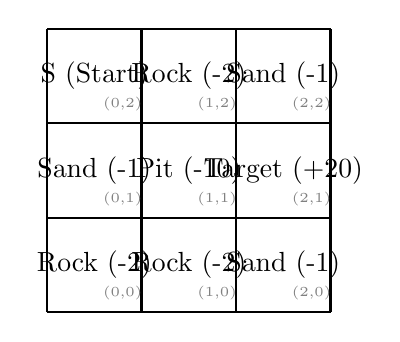
\begin{tikzpicture}[scale=1.2]
    \draw[thick] (0,0) grid (3,3);
    \node at (0.5, 2.5) {S (Start)};
    \node at (1.5, 2.5) {Rock (-2)};
    \node at (2.5, 2.5) {Sand (-1)};
    \node at (0.5, 1.5) {Sand (-1)};
    \node at (1.5, 1.5) {Pit (-10)};
    \node at (2.5, 1.5) {Target (+20)};
    \node at (0.5, 0.5) {Rock (-2)};
    \node at (1.5, 0.5) {Rock (-2)};
    \node at (2.5, 0.5) {Sand (-1)};
    \foreach \x in {0,1,2} \foreach \y in {0,1,2} \node[font=\tiny, gray] at (\x+0.8, \y+0.2) {(\x,\y)};
\end{tikzpicture}
\end{center}
\textbf{Task:} Perform one iteration of Value Iteration for state $(1,2)$ [Rock].
Current Estimates $V_k$: $V_k(0,2)=5.0$, $V_k(2,2)=8.0$, $V_k(1,1)=-5.0$. All others 0 (except Target=0).
Transition: 0.8 Success, 0.1 Slip Left, 0.1 Slip Right. $\gamma=0.9$.
Reward depends on destination terrain.
\end{problem}

\begin{solution}
Calculations detailed in previous section.
$Q(\text{Right}) = 3.49$.
$V_{k+1}(1,2) = 3.49$.
\end{solution}
\newpage

% --- Problem 3: MC vs TD ---
\begin{problem}{Casino Blackjack (First-Visit MC vs TD(0))}
\textbf{Scenario:}
Episodes:
1. $19 \to 20 \to 21 \to \text{Win (+1)}$
2. $19 \to 18 \to \text{Lose (-1)}$
3. $20 \to \text{Lose (-1)}$
\textbf{Task:} Calculate $V(19)$ using MC and TD(0).
\end{problem}
\begin{solution}
$V_{MC}(19) = 0$.
$V_{TD}(19) = 0$.
\end{solution}
\newpage

% --- Problem 4: DQN ---
\begin{problem}{Highway Lane Changing (Double DQN Target)}
\textbf{Scenario:}
An autonomous vehicle uses a Deep Q-Network.
\begin{center}
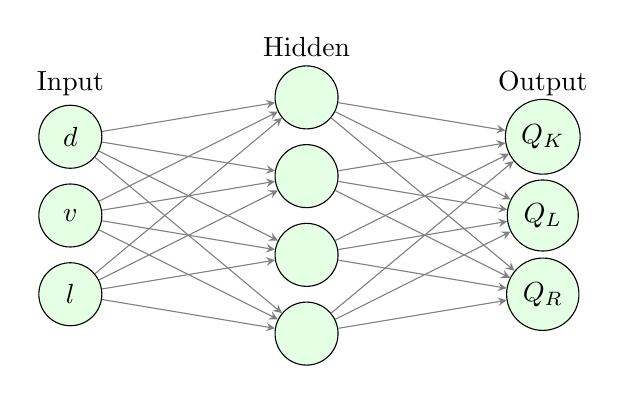
\begin{tikzpicture}[x=1.5cm, y=1.0cm]
    % Input
    \node[netnode] (i1) at (0, 2) {$d$};
    \node[netnode] (i2) at (0, 1) {$v$};
    \node[netnode] (i3) at (0, 0) {$l$};
    \node[above] at (0, 2.4) {Input};

    % Hidden
    \node[netnode] (h1) at (2, 2.5) {};
    \node[netnode] (h2) at (2, 1.5) {};
    \node[netnode] (h3) at (2, 0.5) {};
    \node[netnode] (h4) at (2, -0.5) {};
    \node[above] at (2, 2.9) {Hidden};

    % Output
    \node[netnode] (o1) at (4, 2) {$Q_K$};
    \node[netnode] (o2) at (4, 1) {$Q_L$};
    \node[netnode] (o3) at (4, 0) {$Q_R$};
    \node[above] at (4, 2.4) {Output};

    % Connections
    \foreach \i in {i1,i2,i3} \foreach \h in {h1,h2,h3,h4} \draw[arrow, thin, gray] (\i) -- (\h);
    \foreach \h in {h1,h2,h3,h4} \foreach \o in {o1,o2,o3} \draw[arrow, thin, gray] (\h) -- (\o);
\end{tikzpicture}
\end{center}
Outputs for $s_{t+1}$:
Online: Keep(4.5), Left(5.2), Right(4.9).
Target: Keep(4.8), Left(3.9), Right(5.0).
Reward $r=-0.5, \gamma=0.95$.
\textbf{Task:} Calculate Standard DQN vs Double DQN Target.
\end{problem}

\begin{solution}
\textbf{Standard DQN:} Max Target = 5.0. $Y = -0.5 + 0.95(5.0) = 4.25$.
\textbf{Double DQN:} Max Online Action = Left. Target Value for Left = 3.9. $Y = -0.5 + 0.95(3.9) = 3.205$.
\end{solution}
\newpage

% --- Problem 5: PER ---
\begin{problem}{Robotic Arm Grip Failure (Prioritized Replay)}
\textbf{Scenario:}
Prioritized Replay Buffer. $p_i = 0.1, \alpha=0.6, \beta=0.4, N=10000$.
Sample sum = 100.
TD Error $\delta = 2.0$.
\end{problem}

\begin{solution}
$P(i) = 0.00251$.
$w_i \approx 0.275$.
$p_{new} \approx 2.0$.
\end{solution}
\newpage

% --- Problem 6: Policy Gradient ---
\begin{problem}{Drone Stabilization (Continuous Policy Gradient)}
\textbf{Scenario:}
Gaussian Policy $\pi(a|s) = \mathcal{N}(\mu, \sigma^2)$.
\begin{center}
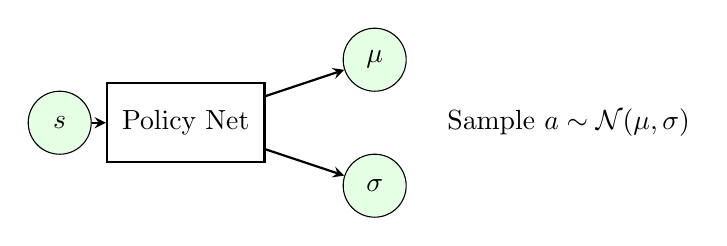
\begin{tikzpicture}[scale=0.8]
    \node[netnode] (s) at (0,0) {$s$};
    \node[box] (net) at (2,0) {Policy Net};
    \node[netnode] (mu) at (5, 1) {$\mu$};
    \node[netnode] (sigma) at (5, -1) {$\sigma$};

    \draw[arrow] (s) -- (net);
    \draw[arrow] (net) -- (mu);
    \draw[arrow] (net) -- (sigma);

    \node[right] at (6, 0) {Sample $a \sim \mathcal{N}(\mu, \sigma)$};
\end{tikzpicture}
\end{center}
$\mu=5.0, \sigma=1.0$. Sample $a=6.5$. Advantage $A=2.0$.
\textbf{Task:} Update $\mu$.
\end{problem}

\begin{solution}
$\nabla_\mu \ln \pi = \frac{a-\mu}{\sigma^2} = 1.5$.
$\mu_{new} = 5.0 + 0.1(2.0)(1.5) = 5.3$.
\end{solution}
\newpage

% --- Problem 7: Actor-Critic ---
\begin{problem}{Server Load Balancing (A2C Update)}
\textbf{Scenario:}
Actor-Critic. $V(s_t)=5.0, V(s_{t+1})=6.0, r=10$.
$\pi(a_t|s_t)=0.4$.
\textbf{Task:} Calculate Critic and Actor Loss.
\end{problem}

\begin{solution}
$\delta_t = 10.4$.
$L_{critic} = 54.08$.
$L_{actor} = 9.526$.
\end{solution}
\newpage

% --- Problem 8: PPO ---
\begin{problem}{Bipedal Walker (PPO Clipping)}
\textbf{Scenario:}
PPO Clip $\epsilon=0.2$.
Case 1: $A=1.5, \pi_{old}=0.2, \pi_{new}=0.3$.
Case 2: $A=-1.5, \pi_{old}=0.2, \pi_{new}=0.1$.
\end{problem}

\begin{solution}
Case 1: Ratio 1.5. Clipped to 1.2. Objective 1.8.
Case 2: Ratio 0.5. Clipped to 0.8? No, min is -1.2.
\end{solution}
\newpage

% --- Problem 9: Dueling DQN ---
\begin{problem}{Fighting Game AI (Dueling Architecture)}
\textbf{Scenario:}
Dueling DQN Architecture.
\begin{center}
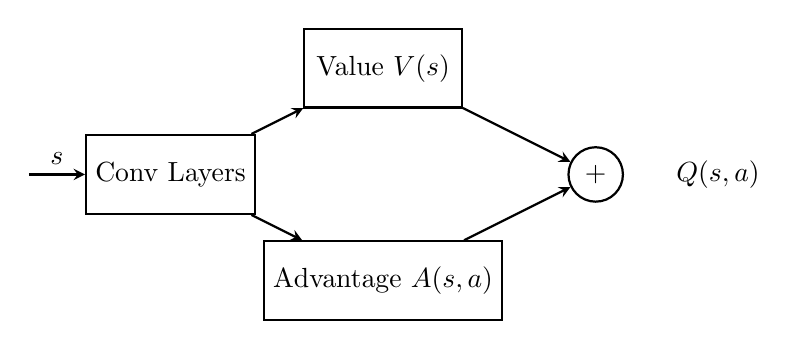
\begin{tikzpicture}[scale=0.9]
    \node[box] (conv) at (0,0) {Conv Layers};
    \node[box] (v) at (3, 1.5) {Value $V(s)$};
    \node[box] (a) at (3, -1.5) {Advantage $A(s,a)$};
    \node[circle, draw, thick] (plus) at (6, 0) {$+$};
    \node[right] at (7,0) {$Q(s,a)$};

    \draw[arrow] (-2,0) -- node[above] {$s$} (conv);
    \draw[arrow] (conv) -- (v);
    \draw[arrow] (conv) -- (a);
    \draw[arrow] (v) -- (plus);
    \draw[arrow] (a) -- (plus);
\end{tikzpicture}
\end{center}
$V=20.0, A=[2.0, 5.0, -1.0]$.
\textbf{Task:} Calculate $Q(\text{Kick})$ using Mean Aggregation.
\end{problem}

\begin{solution}
Mean $A = 2.0$.
$Q(\text{Kick}) = 20.0 + (5.0 - 2.0) = 23.0$.
\end{solution}
\newpage

% --- Problem 10: MCTS ---
\begin{problem}{Board Game Strategy (MCTS Step)}
\textbf{Scenario:}
MCTS Iteration.
\begin{center}
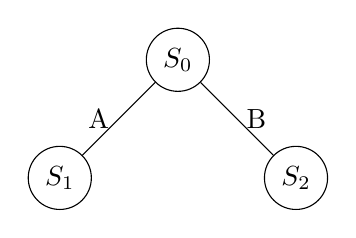
\begin{tikzpicture}[level distance=1.5cm,
  level 1/.style={sibling distance=3cm},
  level 2/.style={sibling distance=1.5cm}]
  \node[circle, draw] {$S_0$}
    child {node[circle, draw] {$S_1$} edge from parent node[left] {A}}
    child {node[circle, draw] {$S_2$} edge from parent node[right] {B}};
\end{tikzpicture}
\end{center}
$S_1 (8/10), S_2 (6/10)$. $N_{root}=20$. $C=1.4$.
\textbf{Task:} Select, Expand, Simulate (+1), Backup.
\end{problem}

\begin{solution}
Select $S_1$ (UCB 1.566 vs 1.366).
Update $S_1 \to 9/11$. $S_0 \to N=21$.
\end{solution}

\end{document}
